\section{Architetture dei Modelli CNN}
\subsection{LeNet5}

LeNet5 è stata una delle prima architetture di reti convolutive. LeNet5 fu introdotta da Yann LeCun 
nel 1998 e aveva come applicazione principale quello di riconoscre i caratteri scritti a mano.
La struttura si componeva di due layer convoluzionali, due sottostrati di campionamento
posti dopo il livello convolutivo e 2 layer fully connected seguiti da un layer di output con
connessione Gaussiana.

\begin{figure}[H]
    \centering
    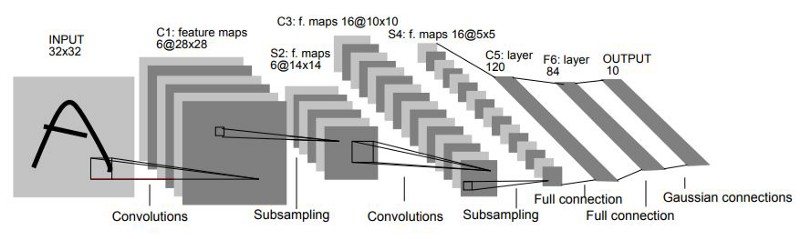
\includegraphics[width=1\textwidth]{Immagini/Generiche/LaNet5.jpeg}
    \caption{Classica architettura di LeNet}
    \label{fig:LaNet5}
    %Figura 2.1: Esempio schematico di un neurone
\end{figure}


\subsection{AlexNet}
AlexNet è un'architettura di rete neurale convolutiva (CNN) introdotta nel 2012 da Alex 
Krizhevsky, Ilya Sutskever e Geoffrey Hinton.
Ha rivoluzionato il campo della visione artificiale vincendo la competizione ImageNet Large Scale 
Visual Recognition Challenge (ILSVRC) del 2012 con un notevole margine rispetto ai concorrenti, 
dimostrando per la prima volta l'enorme potenziale delle reti profonde (deep learning) nell'elaborazione 
delle immagini.
La struttura prevedeva un primo livello che si occupasse della convoluzione e del Max
Pooling, implementato con LRN (Local Response Normalization): erano stati usati 96
differenti filtri recettivi, di dimensione 11x11; nel secondo livello con filtri 5x5 era svolta
la medesima operazione. Nel terzo, quarto e quinto erano usati filtri 3x3 ma con rispetti-
vamente 384, 384, 296 feature map per l’operazione di convoluzione che era seguita dalla
funzione di Relu. Infine, i due fully layer erano usati con funzione softmax.

\begin{figure}[H]
    \centering
    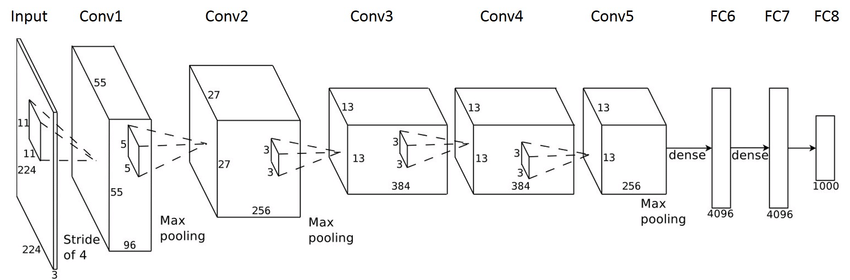
\includegraphics[width=1\textwidth]{Immagini/Generiche/AlexNet.png}
    \caption{Classica architettura di AlexNet}
    \label{fig:AlexNet}
    %Figura 2.1: Esempio schematico di un neurone
\end{figure}

\subsection{VGG-Net}